\section{Exercise one}

Consider the process described by the expression:
\[y(t)=\dfrac{1}{2}y(t-1)+e(t)-e(t-1) \qquad e(t) \sim WN(0,9)\]
Determine the spectral density function of the provided process.

\subsection*{Solution}
For a stationary stochastic process, the following formula holds:
\[\Gamma_y(\omega)=\left\lvert W(e^{j\omega})\right\rvert^2 \Gamma_u(\omega) = \left\lvert W(e^{j\omega})\right\rvert^2 \lambda^2\]

We start by computing the transfer function:
\[y(t)=\dfrac{z-1}{z-\frac{1}{2}}\]
Since the pole is inside the unit circle and $e(t)$ is a stationary stochastic process ( White Noise), $y(t)$ is also a stationary stochastic process.
We can then use the fundamental theorem of spectral analysis:
\[\Gamma_y(\omega) = \left\lvert \dfrac{e^{j\omega}-1}{e^{j\omega}-\frac{1}{2}}\right\rvert^2 9\]
We compute the squares as follows:
\begin{itemize}
    \item $\left\lvert e^{j\omega}-1 \right\rvert^2=\left( e^{j\omega}-1 \right)\left( e^{-j\omega}-1 \right)=2(1-\cos\omega)$
    \item $\left\lvert e^{j\omega}-\frac{1}{2}\right\rvert^2=\left( e^{j\omega}-\frac{1}{2} \right)\left( e^{-j\omega}-\frac{1}{2} \right)=\dfrac{5}{4}-\cos\omega$
\end{itemize}
Thus, the spectral density function is:
\[\Gamma_y(\omega) = \dfrac{1-\cos\omega}{\frac{5}{4}-\cos\omega} 18\]
This allows us to generate the graph:
\begin{figure}[H]
    \centering
    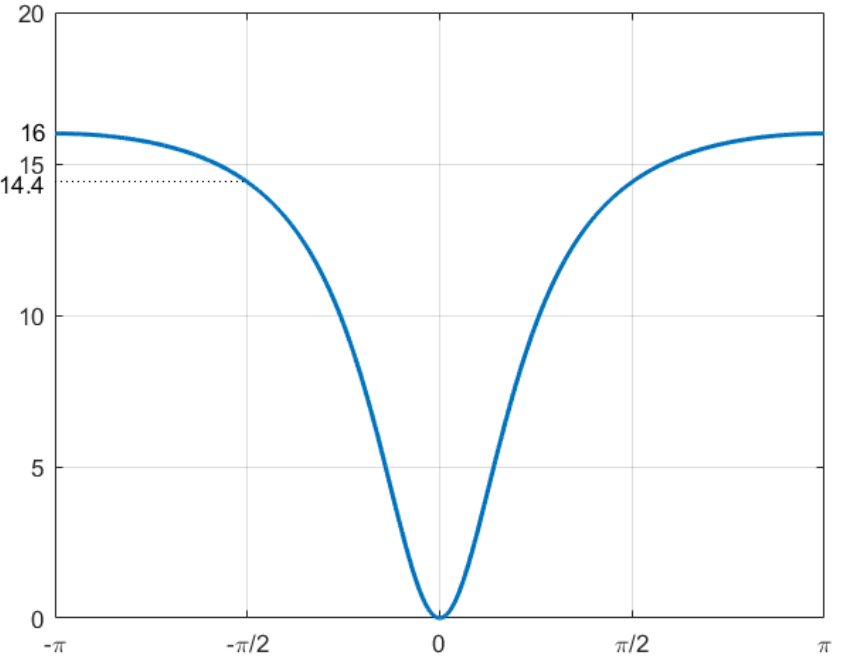
\includegraphics[width=0.4\linewidth]{images/spec.png}
\end{figure}